\chapter{Systems of Linear Equations and Matrices}\label{Chapter:Matrices}


\section*{Introduction}

In this chapter, we introduce the notion of Linear Systems.  Linear Systems occur whenever we have collections of variables with linear relations with each other.  For example, we may want to eat a diet which contains certain levels of protein and fiber, and we wonder how much chicken and kale we should eat to achieve this?  Or we have Business, English and Math students, each of whom take different number of these courses, if we knew how many of each major there were, could we compute how many credits of each type of course would be taught?  This chapter will focus on the techniques and tools to model and address these types of situations.



\section{Systems of Linear  Equations}\label{Section:SystemsofEquations}

A system of equations with unknowns $x_1,\ldots,x_n$ is a collection of first degree equations:

\begin{eqnarray*}
a_{1,1}x_1+a_{1,2}x_2+\cdots+a_{1,n}x_n&=&b_1\\
a_{2,1}x_1+a_{2,2}x_2+\cdots+a_{2,n}x_n&=&b_1\\
\vdots &=&\vdots\\
a_{m,1}x_1+a_{m,2}x_2+\cdots+a_{m,n}x_n&=&b_1\\
\end{eqnarray*}



\subsection{What Exactly is  a Solution to a System of Linear Equations?}

To answer the question that is the name of this section, we should kinda back up here and ask ``What is a solution to an equation?"\\

For example, what is a solution to $y=2x+3$? After dealing with linear equations in Chapter 1, we should have some sense as to what $y=2x+3$ looks like, that is a line with slope 2 and $y$-intercept $(0,3)$.  But what IS this line?  It's the collection of all points $(x,y)$ that make the above equation true.  So $(0,3), (-1,1)$ and $(2,7)$ are all on this line because they make the equation true ($3=2(0)+3, 1=2(-1)+3, 7=2(2)+3$).  A point like $(1,1)$ is NOT on this line because $1\neq 2(1)+3$.  \\

So a solution to an equation is \textbf{any point which makes the equation true}.\\

A \textit{System of Equations} is a collection of equations.  Thus, a solution to a system of equations is \textbf{any point which makes \underline{all} the equations true}.

\subsection{What are the Types of Solutions that we can have?}

So a solution to the system:

\begin{eqnarray*}
2x+3y&=&15\\
x-y&=&0
\end{eqnarray*}
is a collection of points that satisfy the first AND the second linear equalities.  The first equation describes the line: $y=-\frac{2}{3}x+5$, whereas the second describes the line $y=x$.  Each of these equations represent lines, so each individually has infinitely many solutions.  The question is, how many solutions do these lines have in common?\\

There are a number of ways to find out, but the most straight forward is simply to graph the system:

$$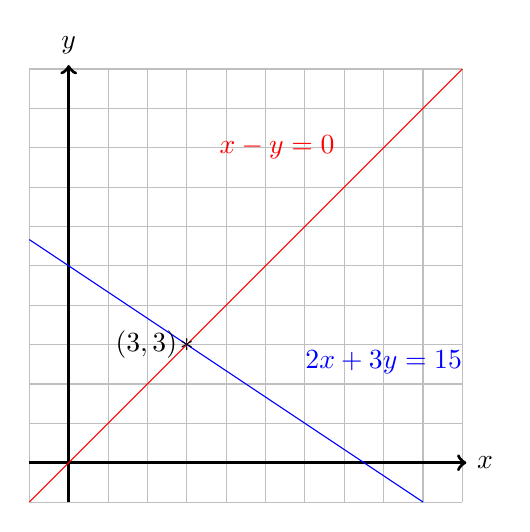
\begin{tikzpicture}[scale=0.5][domain=-1:10]
    \draw[gray!50, thin, step=1] (-1,-1) grid (10,10);
    \draw[very thick,->] (-1,0) -- (10.1,0) node[right] {$x$};
    \draw[very thick,->] (0,-1) -- (0,10.1) node[above] {$y$};

%    \foreach \x in {0,...,11} \draw (\x,0.05) -- (\x,-0.05) node[below] {\tiny\x};
%    \foreach \y in {0,...,28} \draw (-0.05,\y) -- (0.05,\y) node[right] {\tiny\y};


    \draw[scale=1,domain=-1:9,smooth,variable=\x,blue] plot ({\x},{(-2/3)*\x+5});
   \draw[scale=1,domain=-1:10,smooth,variable=\x,red] plot ({\x},{\x});

\node at (3,3){$*$};
\draw (3,3) --node[left]{$(3,3)$}(3,3);
\draw[blue] (8,2) --node[above]{$2x+3y=15$}(8,2);
\draw[red] (7,8) --node[left]{$x-y=0$}(7,8);



\end{tikzpicture}$$   


\url{https://www.desmos.com/calculator/cdrgyxm2al}.

As one can see, although each line has infinitely many points, the only solution they have in common is the point $(3,3)$.  To verify this, we note that $2(3)+3(3)=15$ and $3-3=0$, so both equations are satisfied.  This system has \textbf{a unique solution}\\

What else could happen when solving a system of equations?  Well, consider:


\begin{eqnarray*}
x+y&=&5\\
2x+2y&=&10.
\end{eqnarray*}

If we look at the graph of both lines, we only see one actual line:
 $$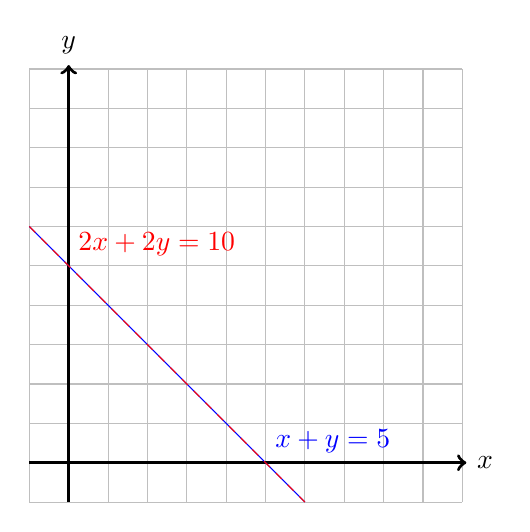
\begin{tikzpicture}[scale=0.5][domain=-1:10]
    \draw[gray!50, thin, step=1] (-1,-1) grid (10,10);
    \draw[very thick,->] (-1,0) -- (10.1,0) node[right] {$x$};
    \draw[very thick,->] (0,-1) -- (0,10.1) node[above] {$y$};

%    \foreach \x in {0,...,11} \draw (\x,0.05) -- (\x,-0.05) node[below] {\tiny\x};
%    \foreach \y in {0,...,28} \draw (-0.05,\y) -- (0.05,\y) node[right] {\tiny\y};


    \draw[scale=1,domain=-1:6,smooth,variable=\x,blue] plot ({\x},{(-1)*\x+5});
   \draw[scale=1,domain=-1:6,smooth,variable=\x,red, dashed] plot ({\x},{-1*\x+5});


\draw[blue] (5,0) --node[above right]{$x+y=5$}(5,0);
\draw[red] (0,5) --node[above right]{$2x+2y=10$}(0,5);


\end{tikzpicture}$$   


\url{https://www.desmos.com/calculator/oaqbrkruhl}. 

This is because both equations describe the same line.  After all, whenever $x+y=5$, it would have to be true that $2(x+y)=5\cdot2$ and thus $2x+2y=10$.  So ANY point that is a solution to one equation is a solution to the other, this system has \textbf{infinitely many solutions}.\\

Another possibility arises from the following example:


\begin{eqnarray*}
x+y&=&5\\
x+y&=&6\end{eqnarray*}

If we graph these lines side by side:

$$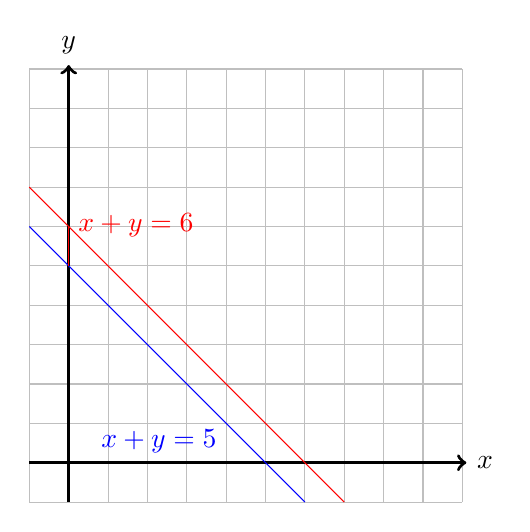
\begin{tikzpicture}[scale=0.5][domain=-1:10]
    \draw[gray!50, thin, step=1] (-1,-1) grid (10,10);
    \draw[very thick,->] (-1,0) -- (10.1,0) node[right] {$x$};
    \draw[very thick,->] (0,-1) -- (0,10.1) node[above] {$y$};

%    \foreach \x in {0,...,11} \draw (\x,0.05) -- (\x,-0.05) node[below] {\tiny\x};
%    \foreach \y in {0,...,28} \draw (-0.05,\y) -- (0.05,\y) node[right] {\tiny\y};


    \draw[scale=1,domain=-1:6,smooth,variable=\x,blue] plot ({\x},{(-1)*\x+5});
   \draw[scale=1,domain=-1:7,smooth,variable=\x,red] plot ({\x},{-1*\x+6});


\draw[blue] (4,0) --node[above left]{$x+y=5$}(4,0);
\draw[red] (0,6) --node[above right]{$x+y=6$}(0,5);


\end{tikzpicture}$$   


\url{https://www.desmos.com/calculator/djqxxge4ce}. 

We can see that these lines are parallel and do not actually have any points in common.  After all, how many pairs of numbers $x$ and $y$ sum to both 5 AND 6?  It should be clear that this system has \textbf{no solutions}.\\

Of course, these have all been Systems of Linear Equations in 2 variables.  When we increase the number of variables, we increase the dimensionality of the potential solution space, and what it means to be ``linear" changes somewhat.  Nevertheless, these examples illustrate the 3 possible outcomes of a system of linear equations in any dimension:

\begin{itemize}
\item There is a unique Solution.
\item There are infinitely many Solutions.
\item There are no Solutions.
\end{itemize}



\subsection{How do we find the Solution(s)/know we have No Solutions?}

In 2 variables, it's simple enough we can just graph, as we did above.  But we should try to develop some algebraic techniques as well, since this will be harder to do when we increase the dimensions of our problems.\\


What we introduce here is the Echelon Method, the general goal is to take non-zero multiples of our equations and use them to eliminate variables in the other equations so that a solution to a variable can be made known.  This process should also reveal if there are infinitely many or no solutions.\\


\begin{example}
\begin{eqnarray*}
2x+3y&=&1\\
x+y&=&0
\end{eqnarray*}

We note that whatever the solutions to this are, they should be the same as the solutions to:

\begin{eqnarray*}
x+\frac{3}{2}y&=&\frac{1}{2}\\
x+y&=&0
\end{eqnarray*}

We've divided the first equation in half, but we haven't actually changed what points will make that equation true.  Then:

\begin{eqnarray*}
x+\frac{3}{2}y&=&\frac{1}{2}\\
x+y-(x+\frac{3}{2}y)&=&0-\frac{1}{2}
\end{eqnarray*}

Must also be true, since we can add and subtract the same values from 2 sides of an equation and preserve the solutions.  By doing this, we kill off the $x$ in the second equation and we can solve for $y$:

\begin{eqnarray*}
x+\frac{3}{2}y&=&\frac{1}{2}\\
-\frac{1}{2}y&=&-\frac{1}{2}
\end{eqnarray*}

So $y=1$ based on the second line.  

\begin{eqnarray*}
x+\frac{3}{2}y&=&\frac{1}{2}\\
y&=&1
\end{eqnarray*}


If we take $-\frac{3}{2}$ times the second line and add it to the first:

\begin{eqnarray*}
x+\frac{3}{2}y-\frac{3}{2}(y)&=&\frac{1}{2}-\frac{3}{2}(1)\\
y&=&1
\end{eqnarray*}

We obtain:

\begin{eqnarray*}
x&=&-1\\
y&=&1
\end{eqnarray*}

We can verify that if we consider the original system:


\begin{eqnarray*}
2x+3y&=&1\\
x+y&=&0
\end{eqnarray*}
 then by evaluating at $x=-1, y=1$:
 
\begin{eqnarray*}
2(-1)+3(1)=-2+3&=&1\\
-1+1&=&0
\end{eqnarray*}
 


\end{example}

\begin{example} So if we consider:

\begin{eqnarray*}
x+y&=&2\\
2x+2y&=&4.
\end{eqnarray*}

Just like before, we want to kill the $x$ in the second equation:

\begin{eqnarray*}
x+y&=&2\\
2x+2y-2(x+y)&=&4-2(2).
\end{eqnarray*}

Which gives us:

\begin{eqnarray*}
x+y&=&2\\
0&=&0.
\end{eqnarray*}

Well..., certainly that second line doesn't contribute much, zero is always equal to itself.  So the solutions are just whenever $x+y=2$, which happens for infinitely many possible pairs.


\end{example}

\begin{example}


 Lastly, when we look at:

\begin{eqnarray*}
x+y&=&0\\
x+y&=&1.
\end{eqnarray*}

We can try to kill the $x$ in the second line as before:

\begin{eqnarray*}
x+y&=&0\\
x+y-(x+y)&=&1-0.
\end{eqnarray*}

Where we get:

\begin{eqnarray*}
x+y&=&0\\
0&=&1.
\end{eqnarray*}

So all you have to do is find a pair $(x,y)$ so that $0=1$... which is not ever going to happen.  So this will never have a solution.


\end{example}



\section{Representing a System of Linear Equations as a Matrix}\label{Section:SystemasMatrix}

Given a system of equations, we can try to encode that information in a matrix:

So for example the system of equations:

\begin{eqnarray*}
2x+3y+z&=&3\\
-2x+4y+2z&=&0\\
x-y+2z&=&3
\end{eqnarray*}

Would have matrix representation:

$$ \left( \begin{array}{rrr|r}
2 & 3 & 1& 3\\
-2 & 4 & 2 & 0\\
1 & -1 & 2 & 3
\end{array}\right).$$

A \textbf{matrix} is a rectangular array of numbers, each number is an \textbf{entry} of the matrix.  In the above example, the vertical line is a visual reminder to separate the constant terms from the variables.  A matrix displayed this way is an \textbf{augmented matrix}.

By letting each column of a matrix represent a different variable or constant and arranging the linear equations into rows, one can write any linear system of equations as an augmented matrix.   Conversely, if you have a matrix:

$$ \left( \begin{array}{rr|r}
1 & 2 & 4\\
3 & 3  & 9\\
\end{array}\right)$$

This represent the system of equations:


\begin{eqnarray*}
x+2y&=&4\\
3x+3y&=&9
\end{eqnarray*}

\subsection{Solving Systems of Linear Equations}

So let's consider the above system/matrix:

$$ \left( \begin{array}{rr|r}
1 & 2 & 4\\
3 & 3  & 9\\
\end{array}\right)$$



We are allowed to manipulate this matrix in a number of ways.  Remembering that each row represents a linear equation:

\begin{enumerate}
\item \textbf{You can multiply any row by a non-zero multiple}.\\ 

We can do this because say, the solutions to $x+2y=4$ are the same as the solutions to $-x-2y=-4$ or $2x+4y=8$, so we're not adding in new solutions or removing existing solutions.

\item \textbf{You can add to any row, the multiple of any row.}\\

Adding a linear equality to another linear equality preserves the solutions to both equations.

\item \textbf{You can rearrange the rows.}\\

The solutions to a system of equations does not depend on the order in which they appear.

\end{enumerate}


So our goal here is to change this system into one where it's much easier to see what the solution is.  The best way to do this, is to not have all these x's and y's, I want 2 equations: $x=?, y=??$.

So:

\begin{eqnarray*}
\left( \begin{array}{rr|r}
1 & 2 & 4\\
3 & 3  & 9\\
\end{array}\right)&&\\
(1/3)R_2\mapsto R_2 \left( \begin{array}{rr|r}
1 & 2 & 4\\
1 & 1  & 3\\
\end{array}\right)&&\\
(-1)R_1+R_2\mapsto R_2 \left( \begin{array}{rr|r}
1 & 2 & 4\\
0 & -1  & -1\\
\end{array}\right)&&\\
(-1)R_2\mapsto R_2 \left( \begin{array}{rr|r}
1 & 2 & 4\\
0 & 1  & 1\\
\end{array}\right)&&\\
(-2)R_2+R_1\mapsto R_1 \left( \begin{array}{rr|r}
1 & 0 & 2\\
0 & 1  & 1\\
\end{array}\right)&&\\
\end{eqnarray*}





What system of equations of this?  It is:

\begin{eqnarray*}
x+0y&=&2\\
0x+y&=&1
\end{eqnarray*}

Which must mean: $x=2, y=1$, alright!  By the way, one can test your answers to see if they are correct!

$$1(2)+2(1)=4, 3(1)+3(2)=9$$ so it checks out.

A matrix with 1's across the diagonal, and 0's above and below these 1's (as above) is called \textbf{reduced row-echelon form}.  A process to obtain a reduced row echelon form matrix  is called the \textbf{Gauss-Jordan Method}.  The methodology is:

\begin{enumerate}
    \item Starting with the first row, multiply by a number so it's leading (leftmost) value is 1.
    \item Multiply and add copies of this row to all rows below so that every entry below this leading 1 is a 0.
    \item Repeat steps (1) and (2) for subsequent rows until the last row.
    \item Starting with the bottom row working up, repeat steps (1)-(3) except working upwards and making entries \textbf{above} the leading 1's 0.
\end{enumerate}

\begin{example}\label{Example:GaussJordan}
Solve the linear system:

\begin{eqnarray*}
3x+2y+z&=&1\\
x+y-z&=&3\\
2x-y+2z&=&-2\\
\end{eqnarray*}

This corresponds to augmented matrix:


$$\left( \begin{array}{rrr|r}
3 & 2 & 1 & 1\\
1 & 1  & -1 & 3\\
2 & -1 & 2 & -2
\end{array}\right)$$

So applying Gauss-Jordan:

\begin{eqnarray*}
\frac{1}{3}R_1\to R_1 \left( \begin{array}{rrr|r}
3 & 2 & 1 & 1\\
1 & 1  & -1 & 3\\
2 & -1 & 2 & -2
\end{array}\right)&&\\
\frac{1}{3}R_1\to R_1 \left( \begin{array}{rrr|r}
1 & \frac{2}{3} & \frac{1}{3} & \frac{1}{3}\\
1 & 1  & -1 & 3\\
2 & -1 & 2 & -2
\end{array}\right)&&\\
-1R_1+R_2\to R_2\left( \begin{array}{rrr|r}
1 & \frac{2}{3} & \frac{1}{3} & \frac{1}{3}\\
0 & -\frac{1}{3}  & -\frac{4}{3} & \frac{8}{3}\\
2 & -1 & 2 & -2
\end{array}\right)&&\\
-3R_2\to R_2\left( \begin{array}{rrr|r}
1 & \frac{2}{3} & \frac{1}{3} & \frac{1}{3}\\
0 & 1  & 4 & -8\\
2 & -1 & 2 & -2
\end{array}\right)&&\\
-2R_1+R_3\to R_3\left( \begin{array}{rrr|r}
1 & \frac{2}{3} & \frac{1}{3} & \frac{1}{3}\\
0 & 1  & 4 & -8\\
0 & -\frac{7}{3} & \frac{4}{3} & -\frac{8}{3}
\end{array}\right)&&\\
\frac{3}{7}R_2+R_3\to R_3\left( \begin{array}{rrr|r}
1 & \frac{2}{3} & \frac{1}{3} & \frac{1}{3}\\
0 & 1  & 4 & -8\\
0 & 0 & \frac{64}{21} & -\frac{128}{21}
\end{array}\right)&&\\
\frac{21}{64}R_3\to R_3\left( \begin{array}{rrr|r}
1 & \frac{2}{3} & \frac{1}{3} & \frac{1}{3}\\
0 & 1  & 4 & -8\\
0 & 0 & 1 & -2
\end{array}\right)&&\\
\end{eqnarray*}

Then we work from bottom back up:

\begin{eqnarray*}
-4R_3 + R_2\to R_2\left( \begin{array}{rrr|r}
1 & \frac{2}{3} & \frac{1}{3} & \frac{1}{3}\\
0 & 1  & 0 & 0\\
0 & 0 & 1 & -2
\end{array}\right)&&\\
-\frac{1}{3}R_3 + R_1\to R_1\left( \begin{array}{rrr|r}
1 & \frac{2}{3} & 0 & 1\\
0 & 1  & 0 & 0\\
0 & 0 & 1 & -2
\end{array}\right)&&\\
-\frac{2}{3}R_2 + R_1\to R_1\left( \begin{array}{rrr|r}
1 & 0 & 0 & 1\\
0 & 1  & 0 & 0\\
0 & 0 & 1 & -2
\end{array}\right)&&\\
\end{eqnarray*}

Which corresponds to the linear system:


\begin{eqnarray*}
1x+0y+0z&=&1\\
0x+1y+0z&=&0\\
0x+0y+z&=&-2\\
\end{eqnarray*}

Which has solution $x=1, y=0, z=2$.  To verify this works, we can check:

\begin{eqnarray*}
3(1)+2(0)+(-2)&=&1\\
(1)+(0)-(-2)&=&3\\
2(1)-(0)+2(-2)&=&-2\\
\end{eqnarray*}

and we have solved our linear system.


\end{example}

\subsection{Reduced Row Echelon Form using Technology.}

Suppose we wanted to solve the system associated with the augmented matrix:

$$ \left( \begin{array}{rrr|r}
2 & 3 & 1& 3\\
-2 & 4 & 2 & 0\\
1 & -1 & 2 & 3
\end{array}\right).$$

We could solve this the same way we did Example \ref{Example:GaussJordan}, but your first thought here is probably ``I don't want to do this."  Yeah, me neither.  One thing to note is that this process of finding a reduced row echelon form of a matrix is fairly mechanical.  So, we should be able to do this with a machine.

Following this link to an independent sagecell:  \url{https://sagecell.sagemath.org/?z=eJxztM1NLCnKrNAIDNRRiI420jHWMdQxjtWJ1jXSMdEx0jEAMg11dA2BTOPYWE1eroKizLwSDUcES6-oKDVNQ1MTAN6nE6M=&lang=sage}.  You see the following code:

\begin{verbatim}
A=matrix(QQ, [[2,3,1,3],[-2,4,2,0],[1,-1,2,3]])
print(A)
print(A.rref())
\end{verbatim}

The first line defines the matrix $A$ with the rows identical to the rows we defined in our above matrix.  Then the code returns a printout of that matrix, and it's reduced row echelon form:


$$ \left( \begin{array}{rrr|r}
1 & 0 & 0& 1\\
0 & 1 & 0 & 0\\
0 & 0 & 1 & 1
\end{array}\right)$$

So $x=1, y=0, z=1$.  Is this right?  Well, 

\begin{eqnarray*}
2(1)+3(0)+1&=&3\\
-2(1)+4(0)+2(1)&=&0\\
1-0+2(1)&=&3
\end{eqnarray*}

Works for me.

By the way, if you enter the matrix from Example \ref{Example:GaussJordan}, and replace the first line with:

\begin{verbatim}
A=matrix(QQ, [[3,2,1,1],[1,1,1,3],[2,-1,2,-2]])
\end{verbatim}

You should have the reduced row echelon matrix we achieved earlier.






\subsection{Infinitely many solutions}

Consider the system:


\begin{eqnarray*}
x+2y+z&=&3\\
-x+y+0z&=&0\\
0x+3y+z&=&3
\end{eqnarray*}

Then by using rref using as $A$:


\begin{verbatim}
A=matrix(QQ, [[1,2,1,3],[-1,1,0,0],[0,3,1,3]])
\end{verbatim}

We would obtain:


$$ \left( \begin{array}{rrr|r}
1 & 0 & 1/3& 1\\
0 & 1 & 1/3 & 1\\
0 & 0 & 0 & 0
\end{array}\right)$$

Which gives us the system:

\begin{eqnarray*}
x+0y+(1/3)z&=&1\\
0x+y+(1/3)z&=&1\\
0x+0y+0z&=&0\\
\end{eqnarray*}

Well, the last line is useless, it basically says that $0=0$, which is true but useless.  Let's break down the remaining equations:

\begin{eqnarray*}
x+(1/3)z&=&1\\
y+(1/3)z&=&1
\end{eqnarray*}

Which can be thought of as:

\begin{eqnarray*}
x&=&1-(1/3)z\\
y&=&1-(1/3)z
\end{eqnarray*}

So basically what this is saying, no matter what $z$ is, you can fin $x$ and $y$.  So if $z=0$, then $x,y=1$. But if $z=6$, then $x,y=-1$.  Well, what is $z$?  Apparently it can be whatever we want, both of the above triplets provide perfectly legitimate solutions to the original system.  What you see described is a line of solutions.  The 3 equations describe 3 planes in 3 dimensional ($x,y,z)$ space and they intersect at this line which can be describes as the solution to this equation.

\subsection{No Solutions}


Consider a similar system:



\begin{eqnarray*}
x+2y+z&=&3\\
-x+y+0z&=&0\\
0x+3y+z&=&0
\end{eqnarray*}

Then by using rref using as $A$:


\begin{verbatim}
A=matrix(QQ, [[1,2,1,3],[-1,1,0,0],[0,3,1,0]])
\end{verbatim}

We would obtain:


$$ \left( \begin{array}{rrr|r}
1 & 0 & 1/3& 1\\
0 & 1 & 1/3 & 1\\
0 & 0 & 0 & 0
\end{array}\right)$$

Which gives us the system:

\begin{eqnarray*}
x+0y+(1/3)z&=&1\\
0x+y+(1/3)z&=&1\\
0x+0y+0z&=&1\\
\end{eqnarray*}


Well, what does this last line mean?  It says that $0=1$.  When will this happen?  Well basically never, no choice of $x,y,z$ will ever make this true, our 3 planes do not intersect at a point or line or at all, so there is no solution.  


\subsection{Applications}

\begin{example}
A new airline has recently purchased a fleet of Airbus A330-300s, Boeing 767-300ERs, and Boeing Dreamliner 787-9s to meet an estimated demand for 9,300 seats. The A330-300s seat 330 passengers and cost \$250 million each, the 767-300ERs seat 270 passengers and cost \$200 million each, while the 787-9s seat 240 passengers and cost \$250 million each. The total cost of the fleet, which had twice as many 787-9s as 767s, was \$8,100 million. How many of each type of aircraft did the company purchase?\\

It helps perhaps if we organize some of this information in a table.

$$\begin{tabular}{|r||c|c|c||c|}
\hline
& A330-300s &  767-300ERs & 787-9s & Total\\
\hline
\hline
\textbf{Capacity} & 330 & 270 & 240 & \textbf{9,300}\\
\hline
\textbf{Cost (\$ million)} & 250 & 200 & 250 & \textbf{8,100}\\
\hline
\end{tabular}
$$

By letting $x$ denote the numbere of A330-300's, $y$ denote the number of 767-300ERs and $z$ denote the number of 787-9s, we obtain the following linear equalities:

First, the total capacity is 9,300 seats: $$330x+270y+240z=9300.$$

Next, the total cost is \$8,100 million: $$250x+200y+250z=8100.$$

Finally, there are twice as many 787-9s as 767-300ERs: %
\begin{eqnarray*}
z&=&2y\\
-2y+z&=&0.
\end{eqnarray*}

Giving us a system:

\begin{eqnarray*}
330x+270y+240z&=&9300\\
250x+200y+250z&=&8100\\
-2y+z&=&0
\end{eqnarray*}
and corresponding augmented matrix:

$$ \left( \begin{array}{rrr|r}
330 & 270 & 240& 9300\\
250 & 200 & 250 & 8100\\
0 & -2 & 1 & 0
\end{array}\right).$$

Using any method we'd like, we find row reduced echelon form:

$$ \left( \begin{array}{rrr|r}
1 & 0 & 0& 10\\
0 & 1 & 0 & 8\\
0 & 0 & 1 & 16
\end{array}\right)$$

which corresponds to $x=10, y=8, z=16$ or 10 A330-300s, 8 767300ERs and 16 787-9s.

To verify that this is a legitimate solution, check:

\begin{eqnarray*}
330(10)+270(8)+240(16)&=&9300\\
250(10)+200(8)+250(16)&=&8100\\
-2(8)+16&=&0.
\end{eqnarray*}



\end{example}


\begin{example}\label{Example:Vitamin}
Margo needs 200mg of vitamin A, 100mg of vitamin D, and 140mg of vitamin E per week. She has three supplements: the first contains 20\% vitamin A, 20\% vitamin D and 20\%
vitamin E; the second contains 10\% vitamin A, 30\% vitamin D and 40\% vitamin E; the third contains 50\% vitamin A, 10\% vitamin D and 20\% vitamin E. How much of each
supplement should she eat each week?\\

Let $x,y,z$ denote the quantities of supplements 1,2 and 3 she takes each week.  She needs 200mg of vitamin A, which gives us: $$0.2x+0.1y+0.5z=200.$$  Similarly, for 100mg of vitamin D: $$0.2x+0.3y+0.1z=100$$ and for 140mg of vitamin E: $$0.2x+0.2y+0.4z=140.$$

This gives us the system:


\begin{eqnarray*}
0.2x+0.1y+0.5z&=&200\\
0.2x+0.3y+0.1z&=&100\\
0.2x+0.4y+0.2z&=&140
\end{eqnarray*}
 with corresponding matrix:

$$ \left( \begin{array}{rrr|r}
0.2 & 0.1 & 0.5& 200\\
0.2 & 0.3 & 0.1 & 100\\
0.2 & 0.4 & 0.2 & 140
\end{array}\right).$$

This has reduced row echelon form:

$$ \left( \begin{array}{rrr|r}
1 & 0 & 0& 200\\
0 & 1 & 0 & 100\\
0 & 0 & 1 & 300
\end{array}\right)$$

which corresponds to solution $x=200, y=100, z=300$ or 200 mg of supplement 1, 100mg of supplement 2 and 300mg of supplement 3.


\end{example}


\begin{example}

Suppose an event with 300 people ends, and the attendees walk from the venue to two restaurants, Xavier's and Yoneda's. They walk along streets Anderson, Birmingham and Central, which are all one way.  When the night ends, there are 75 people and Xavier's and 225 at Yoneda's.

$$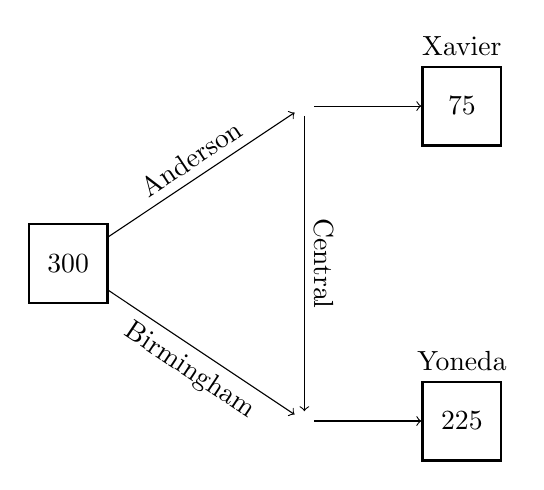
\begin{tikzpicture}
\node (V) at (0,0) [draw,thick,minimum width=1cm,minimum height=1cm] {$300$};

\node (I1) at (3,2) {};
\node (I2) at (3,-2) {};


\draw[->] (V) -- (I1)node[midway,sloped,above]{Anderson};;
\draw[->] (V) -- (I2) node[midway,sloped,below]{Birmingham};
\draw[->] (I1) -- (I2) node[midway,sloped,above]{Central};

\node[label={Xavier}] (X) at (5,2) [draw,thick,minimum width=1cm,minimum height=1cm] {75};

\node[label={Yoneda}] (Y) at (5,-2) [draw,thick,minimum width=1cm,minimum height=1cm] {225};

\draw[->] (I1)--(X);
\draw[->] (I2)--(Y);


\end{tikzpicture}$$

Let $a,b,c$ denote the number of people walking along Anderson, Birmingham and Central.

\begin{enumerate}
    \item Find an expression for the amount of people walking along each street.\\
    
    We first set up our systems of equations.  We first note that all 300 people have to walk either along either Anderson or Birmingham, so $$a+b=300.$$  Next, the 75 at Xavier is the however many people walked down Anderson, and take away whoever veered off onto Central so: $$a-c=75.$$  The 225 people at Yoneda is everyone coming across Birmingham and Central so $$b+c=225.$$  Thus the system is:
    
    \begin{eqnarray*}
    a+b&=&300\\
    a-c&=&75\\
    b+c&=&225,\\
    \end{eqnarray*}
    
    with associated augmented matrix:
    
    $$ \left( \begin{array}{rrr|r}
1 & 1 & 0& 300\\
1 & 0 & -1 & 75\\
0 & 1 & 1 & 225
\end{array}\right).$$
    
So the reduced row echelon form of this is:

    $$ \left( \begin{array}{rrr|r}
1 & 0 & -1 & 75\\
0 & 1 & 1 & 225\\
0 & 0 & 0& 0
\end{array}\right).$$

What this tells us is that there is not a unique solution, as the system associated with this matrix is:

    \begin{eqnarray*}
    a-c&=&75\\
    b+c&=&225,\\
    \end{eqnarray*}

Which is two of the original equations.  So, depending on what $c$ is, this will determine how many people traverse Anderson and Birmingham.

\item If 50 people crossed central, how many people crossed Anderson and Birmingham?\\

So letting $c=50$, we would have:

    \begin{eqnarray*}
    a-c&=&75\\
    a-50&=&75\\
    a&=&125\\
    b+c&=&225\\
    b+50&=&225\\
    b&=&175,
    \end{eqnarray*}
So 125 people across Anderson and 175 across Birmingham.\\

Another way to do this would be to add an equation $c=50$ to our system:

$$ \left( \begin{array}{rrr|r}
1 & 1 & 0& 300\\
1 & 0 & -1 & 75\\
0 & 1 & 1 & 225\\
0 & 0 & 1 & 50
\end{array}\right).$$
    
    Which has reduced row echelon form:
 
 $$ \left( \begin{array}{rrr|r}
1 & 0 & 0 & 125\\
0 & 1 & 0 & 175\\
0 & 0 & 1& 50\\
0 & 0 & 0& 0
\end{array}\right).$$   

That is $a=125, b=125, c=50$ which is our solution above.

\item If 100 people go through Anderson, how many go through Birmingham or Central?\\

We can revisit our linear system from (a):

    \begin{eqnarray*}
    a-c&=&75\\
    100-c&=&75\\
    c&=&25\\
    b+c&=&225\\
    b+25&=&225\\
    b&=&200,
    \end{eqnarray*}
so 200 across Birmingham and 25 across Central.\\

We can also add the linear equation $a=100$:

$$ \left( \begin{array}{rrr|r}
1 & 1 & 0& 300\\
1 & 0 & -1 & 75\\
0 & 1 & 1 & 225\\
1 & 0 & 0 & 100
\end{array}\right)$$

with reduced row echelon form:

$$ \left( \begin{array}{rrr|r}
1 & 0 & 0 & 100\\
0 & 1 & 0 & 200\\
0 & 0 & 1& 25\\
0 & 0 & 0& 0
\end{array}\right).$$  So 100 across Anderson, 200 across Birmingham and 25 across Central.
    
\end{enumerate}



\end{example}

\section{Products and Sums of Matrices}\label{Section:MatrixArithmetic}

In the previous sections, we saw how the entries of matrix may be used to record relationships between two collections of variables.  For example in Example \ref{Example:Vitamin}, the entries in the $3\times 3$ portion of the matrix represents the proportion of vitamins contained by a collection of supplements, with each entry representing a vitamin-supplement pair.  It is natural then, to wonder if we could combine relationships between variables or compose them.  The operations behind these ideas are the sums and products of matrices.

\subsection{Products of Matrices}

We begin with a motivating example:

\begin{example}\label{Example:VitProd}

Recall that in Example \ref{Example:Vitamin} Margo has three supplements: the first contains 20\% vitamin A, 20\% vitamin D and 20\%
vitamin E; the second contains 10\% vitamin A, 30\% vitamin D and 40\% vitamin E; the third contains 50\% vitamin A, 10\% vitamin D and 20\% vitamin E.\\

On Monday she eats 100 mg of supplement 1, 100 mg of supplement 2 and 150 mg of supplement 3.  On Wednesday she eats 150 mg of supplement 1, 50 mg of supplement 2 and 100 mg of supplement 3.  Putting aside that this is an ill advised way to take supplements, how much of each vitamin did she get on each day?\\

We first let $$A= \left( \begin{array}{rrr}
0.2 & 0.1 & 0.5\\
0.2 & 0.3 & 0.1\\
0.2 & 0.4 & 0.2
\end{array}\right)$$

represent the relation between vitamins and supplements, where each row corresponds to vitamins, and each column corresponds to supplements.  So the entry in the second row, second column corresponds to the proportion of supplement 2 which is vitamin D, 30\%.\\

A useful way to conceptualize this matrix is as an arrow or transformation, whose inputs are mg of various supplements, and whose outputs are mg of various vitamins.

$$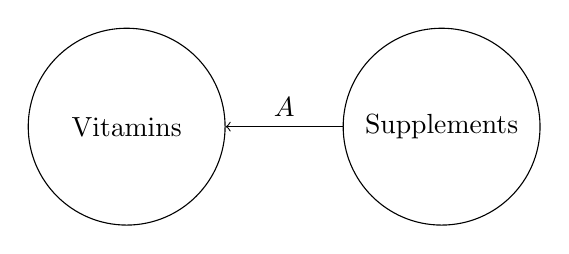
\begin{tikzpicture}
\node(S)[draw,circle,minimum size=2.5cm,inner sep=1pt] at (4,0) {Supplements};
\node(V)[draw,circle,minimum size=2.5cm,inner sep=1pt] at (0,0) {Vitamins};

\draw[->] (S) --node[above]{$A$} (V);

\end{tikzpicture}$$


Next, we record the relationship between days of the week and supplements:

$$B= \left( \begin{array}{rrr}
100 & 150\\
100 & 50\\
150 & 100
\end{array}\right)$$


Where now the rows are quantities of supplements and columns are days of the week.  So the 100 in the third row second column represents the 100mg taken on Wednesday of Supplement 3.  This to may be conceptualized as an arrow or transformation whose inputs are days of the week, and whose outputs are quantities of supplements.

$$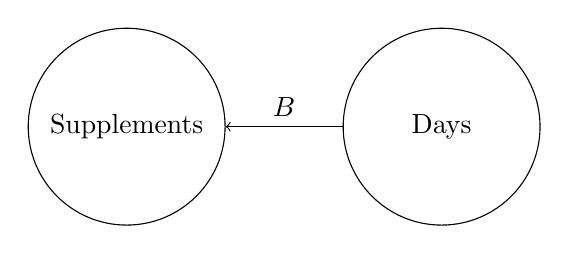
\begin{tikzpicture}
\node(S)[draw,circle,minimum size=2.5cm,inner sep=1pt] at (4,0) {Supplements};
%\node(V)[draw,circle,minimum size=2.5cm,inner sep=1pt] at (0,0) {Vitamins};
\node(D)[draw,circle,minimum size=2.5cm,inner sep=1pt] at (8,0) {Days};

%\draw[->] (S) --node[above]{A} (V);
\draw[->] (D) --node[above]{$B$} (S);

\end{tikzpicture}$$

Our goal now is to establish a relationship between days of the week and quantity of vitamins.

$$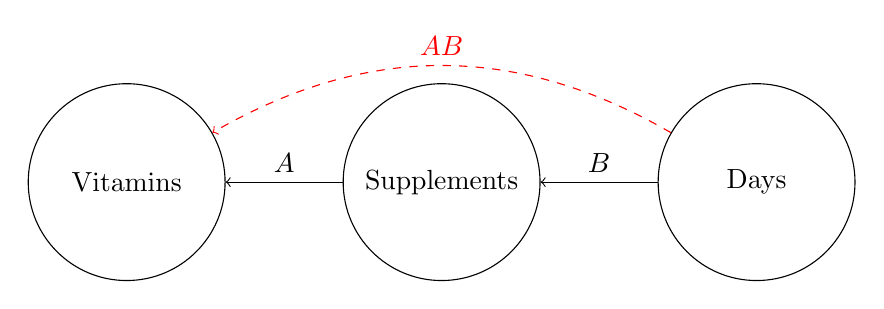
\begin{tikzpicture}
\node(S)[draw,circle,minimum size=2.5cm,inner sep=1pt] at (4,0) {Supplements};
\node(V)[draw,circle,minimum size=2.5cm,inner sep=1pt] at (0,0) {Vitamins};
\node(D)[draw,circle,minimum size=2.5cm,inner sep=1pt] at (8,0) {Days};

\draw[->] (S) --node[above]{$A$} (V);
\draw[->] (D) --node[above]{$B$} (S);

\draw [->, dashed, red] (D) to [out=150,in=30] node[above]{$AB$} (V);


\end{tikzpicture}$$

So, how much Vitamin A does Margo get on Monday?  She took \textcolor{blue}{100} mg of Supplement 1, of which \textcolor{red}{20\%} is Vitamin A, \textcolor{blue}{100} mg of Supplement 2, of which \textcolor{red}{10\%} is Vitamin A, and \textcolor{blue}{150} mg of Supplement 1, of which \textcolor{red}{50\%} is Vitamin A:

$$\left( \begin{array}{rrr}
\textcolor{red}{0.2} & \textcolor{red}{0.1} & \textcolor{red}{0.5}\\
0.2 & 0.3 & 0.1\\
0.2 & 0.4 & 0.2
\end{array}\right)\left( \begin{array}{rrr}
\textcolor{blue}{100} & 150\\
\textcolor{blue}{100} & 50\\
\textcolor{blue}{150} & 100
\end{array}\right)=\left( \begin{array}{cr}
\textcolor{red}{0.2}\cdot\textcolor{blue}{100}+\textcolor{red}{0.1}\cdot\textcolor{blue}{100}+\textcolor{red}{0.5}\cdot\textcolor{blue}{150} & ? \\
? & ? \\
? & ? 
\end{array}\right)=\left( \begin{array}{cr}
105 & ? \\
? & ? \\
? & ? 
\end{array}\right).$$

So on Monday, Margo got 105 mg of vitamin A.  What about the amount of vitamin D she received on Wednesday?  She took \textcolor{blue}{150} mg of Supplement 1, of which \textcolor{red}{20\%} is Vitamin D, \textcolor{blue}{50} mg of Supplement 2, of which \textcolor{red}{30\%} is Vitamin D, and \textcolor{blue}{100} mg of Supplement 1, of which \textcolor{red}{10\%} is Vitamin A:

\begin{eqnarray*}
\left( \begin{array}{rrr}
0.2 & 0.1 & 0.5\\
\textcolor{red}{0.2} & \textcolor{red}{0.3} & \textcolor{red}{0.1}\\
0.2 & 0.4 & 0.2
\end{array}\right)\left( \begin{array}{rrr}
100 & \textcolor{blue}{150}\\
100 & \textcolor{blue}{50}\\
150 & \textcolor{blue}{100}
\end{array}\right)&=&\left( \begin{array}{cr}
105 & ? \\
? & \textcolor{red}{0.2}\cdot\textcolor{blue}{150}+\textcolor{red}{0.3}\cdot\textcolor{blue}{50}+\textcolor{red}{0.1}\cdot\textcolor{blue}{100} \\
? & ? 
\end{array}\right)\\
&=&\left( \begin{array}{cr}
105 & ? \\
? & 55 \\
? & ? 
\end{array}\right).
\end{eqnarray*}

So Margo got 55 mg of Vitamin D on Wednesday.  Following this line of thinking, we obtain matrix:

$$\left( \begin{array}{rrr}
{0.2} & {0.1} & {0.5}\\
0.2 & 0.3 & 0.1\\
0.2 & 0.4 & 0.2
\end{array}\right)\left( \begin{array}{rrr}
{100} & 150\\
{100} & 50\\
{150} & 100
\end{array}\right)=\left( \begin{array}{cr}
105 & 85 \\
65 & 55 \\
90 & 70 
\end{array}\right).$$

This matrix records how much of each vitamin Margo had per day, where vitamins are rows and days are columns.  So on Monday, she got 90 mg of Vitamin E, and on Wednesday, she got 85 mg of Vitamin A.

\end{example}

So with this illustrative example in mind, we can define matrix multiplication.

\begin{definition}\label{Defn:MatrixProd}
For any matrix $M$, let $(M)_{ij}=m_{ij}$ denote the entry in the $i$th row and $j$th column.   Then, given a $m\times n$ matrix $A$ and a $n\times k$ matrix $B$, we define $AB$ the product of $A$ and $B$ to be a $m\times k$ matrix where:

$$(AB)_{ij}=\begin{pmatrix}\textcolor{red}{a_{i1}} & \textcolor{red}{a_{i2}} & \cdots & \textcolor{red}{a_{in}}\end{pmatrix}\begin{pmatrix}\textcolor{blue}{b_{1j}} \\ \textcolor{blue}{b_{2j}} \\ \vdots \\ \textcolor{blue}{b_{nj}}\end{pmatrix}=\begin{pmatrix}\textcolor{red}{a_{i1}}\textcolor{blue}{b_{1j}}+\textcolor{red}{a_{i2}}\textcolor{blue}{b_{2j}}+\cdots+\textcolor{red}{a_{in}}\textcolor{blue}{b_{nj}} \end{pmatrix}$$

\end{definition}

\textbf{Note that the number of columns of $A$ and the number of rows of $B$ must be the same.}  Recall Example \ref{Example:VitProd}, the outputs of $B$ corresponded to the rows, and the inputs of $A$ corresponded to it's columns, so these had to match up.  This number is also the $n$ is Definition \ref{Defn:MatrixProd}.


\begin{example}\label{Example:MoreMatrixProducts}
Let $$A=\begin{pmatrix}
1 & 2 & 3\\ 4 & 5 & 6
\end{pmatrix}, B=\begin{pmatrix}
0.2 & 0.4 \\ 0.5 & 0.6 \\ 0.1 & 0.8
\end{pmatrix}, C=\begin{pmatrix}
10 \\ 20 \\ 15
\end{pmatrix}.$$
Find:

\begin{enumerate}
    \item $AB$.
    \begin{eqnarray*}
    AB=\begin{pmatrix}
1 & 2 & 3\\ 4 & 5 & 6
\end{pmatrix}\begin{pmatrix}
0.2 & 0.4 \\ 0.5 & 0.6 \\ 0.1 & 0.8
\end{pmatrix}&=&\begin{pmatrix}
1\cdot0.2+2\cdot0.5+3\cdot0.1 & 1\cdot0.4+2\cdot0.6+3\cdot0.8\\
4\cdot0.2+5\cdot0.5+6\cdot0.1 & 4\cdot0.4+5\cdot0.6+6\cdot0.8 
\end{pmatrix}\\
&=&\begin{pmatrix}
1.5 & 4 \\ 3.9  &  9.4
\end{pmatrix}
    \end{eqnarray*}
    
    
    
    \item $BA$.
    \begin{eqnarray*}
    BA=\begin{pmatrix}
0.2 & 0.4 \\ 0.5 & 0.6 \\ 0.1 & 0.8
\end{pmatrix}\begin{pmatrix}
1 & 2 & 3\\ 4 & 5 & 6
\end{pmatrix}&=&\begin{pmatrix}
0.2\cdot1+ 0.4\cdot 4 & 0.2\cdot2+ 0.4\cdot 5 & 0.2\cdot3+ 0.4\cdot6\\
0.5\cdot1+ 0.6\cdot 4 & 0.5\cdot2+ 0.6\cdot 5 & 0.5\cdot3+ 0.6\cdot6\\
0.1\cdot1+ 0.8\cdot 4 & 0.1\cdot2+ 0.8\cdot 5 & 0.1\cdot3+ 0.8\cdot6\\
\end{pmatrix}\\
&=&\begin{pmatrix}
1.8 & 2.4 & 3 \\ 2.9  &  4 & 5.1 \\ 3.3 & 4.2 & 5.1
\end{pmatrix}
    \end{eqnarray*}    
    
    \item $AC$.
    \begin{eqnarray*}
    AC=\begin{pmatrix}
1 & 2 & 3\\ 4 & 5 & 6
\end{pmatrix}\begin{pmatrix}
10\\20\\15
\end{pmatrix}&=&\begin{pmatrix}
1\cdot10+2\cdot20+3\cdot15 \\ 4\cdot10+5\cdot20+6\cdot15
\end{pmatrix}\\
&=&\begin{pmatrix}
95 \\ 230
\end{pmatrix}
    \end{eqnarray*}
    
    
    
    \item $CA$.
    
    Notice that if we try to take the product $CA$:
    \begin{eqnarray*}
    CA=\begin{pmatrix}
10\\20\\15
\end{pmatrix}\begin{pmatrix}
1 & 2 & 3\\ 4 & 5 & 6
\end{pmatrix}&=&\begin{pmatrix}
10\cdot1+?\cdot4 & 10\cdot2+?\cdot5 & 10\cdot3+?\cdot6 \\ 20\cdot1+?\cdot4 & 20\cdot2+?\cdot5 & 20\cdot3+?\cdot6\\15\cdot1+?\cdot4 & 15\cdot2+?\cdot5 & 15\cdot3+?\cdot6
\end{pmatrix}
    \end{eqnarray*}
Since the number of columns of the first matrix do not match with the number of rows of the second matrix, the product is not defined.    
    
    \item $BC$.
    
    Since $B$ has 2 columns and $C$ has 3 rows, these values do not match and this product is not defined.
    \item $CB$.
    
    Since $C$ has 1 column and $B$ has 2 rows, these values do not match and this product is not defined.
\end{enumerate}


\end{example}

Something we should observe here is that, unlike products of real numbers, products of matrices are \textbf{NOT} commutative.  In Example \ref{Example:MoreMatrixProducts}, $AB\neq BA$, and $AC$ was defined whereas $CA$ was not.

Another way matrix products deviate from real number products is that the product of matrices whose entries aren't 0 can result in a matrix whose entries are all 0.

\begin{example}
Let $$A=\begin{pmatrix}1&2\\2&4 \end{pmatrix}, B=\begin{pmatrix}2&6\\-1&-3 \end{pmatrix}.$$

Notice that:

\begin{eqnarray*}
AB=\begin{pmatrix}1&2\\2&4 \end{pmatrix}\begin{pmatrix}2&6\\-1&-3 \end{pmatrix}&=&\begin{pmatrix}
1\cdot 2+2\cdot(-1) & 1\cdot 6+2\cdot(-3)\\ 2\cdot 2+4\cdot(-1)&2\cdot 6 +4\cdot(-3)
\end{pmatrix}\\
&=&\begin{pmatrix}
0 & 0 \\ 0 & 0
\end{pmatrix}.
\end{eqnarray*}
Although neither $A$ nor $B$ have 0 entries, their product is an all 0 matrix.  Also notice that this does not mean $BA$ is an all 0 matrix.

\begin{eqnarray*}
BA=\begin{pmatrix}2&6\\-1&-3 \end{pmatrix}\begin{pmatrix}1&2\\2&4 \end{pmatrix}&=&\begin{pmatrix}
2\cdot 1+6\cdot2 & 2\cdot 2+6\cdot4\\ (-1)\cdot 1+(-3)\cdot2&(-1)\cdot 2 +(-3)\cdot4
\end{pmatrix}\\
&=&\begin{pmatrix}
14 & 28 \\ -7 & -14
\end{pmatrix}.
\end{eqnarray*}

\end{example}






\subsection{Sums of Matrices}

Matrix sums are much more straight forward than their products.  Two Matrices need to have the same dimensions in order to be summed, and the sum is just the sum of the entries, so:

$$\begin{pmatrix} a & b \\ c & d \end{pmatrix}+ \begin{pmatrix} w & x \\ y & z \end{pmatrix}=\begin{pmatrix} a+w & b+x \\ c+y & d+z \end{pmatrix}$$


\begin{example}
Company $B$ gets in on this action and will give 2 dollars to each charity for each student who attends.  NOW given $F$ female and $M$ male students, how much money will go to Elderly and the Homeless?

\begin{eqnarray*}
\begin{pmatrix} 0.8 & 0.5 & 0 \\ 0.2 & 0.5 & 1 \end{pmatrix} \left( \begin{pmatrix} 2 & 1 \\ 1 & 2 \\ 2 & 2\end{pmatrix} + \begin{pmatrix} 2 & 2 \\ 2 & 2 \\ 2 & 2\end{pmatrix}   \right)\begin{pmatrix} F\\M \end{pmatrix}&=&\begin{pmatrix} 0.8 & 0.5 & 0 \\ 0.2 & 0.5 & 1 \end{pmatrix} \begin{pmatrix} 4 & 3 \\ 3 & 4 \\ 4 & 4\end{pmatrix} \begin{pmatrix} F\\M \end{pmatrix}\\
&=&\begin{pmatrix} 4.7 & 4.4 \\ 7.3 &  6.6 \end{pmatrix}\begin{pmatrix} F\\M \end{pmatrix}\\
&=&\begin{pmatrix} 4.7F+4.4M\\ 7.3F+6.6M \end{pmatrix}\\
\end{eqnarray*}
So \$$4.7 F+4.4M$ for Elderly and $\$7.3 F+6.6M$ for Homeless.
\end{example}

\section{Computation using Sage}\label{Section:MatrixSage}

As usual, this seems like it should be much easier using technology.  Let's suppose $A=\begin{pmatrix} 1 & 2 \\ 3 & 4\end{pmatrix}, B=\begin{pmatrix} 5 & 6 \\ 7 & 8\end{pmatrix}$.  Verify that:

\begin{eqnarray*}
A+B&=&\begin{pmatrix} 6 & 8 \\ 10 & 12\end{pmatrix}\\
AB&=&\begin{pmatrix} 19 & 22 \\ 43 & 50\end{pmatrix}\\
BA&=&\begin{pmatrix} 23 & 34 \\ 31 & 46\end{pmatrix}
\end{eqnarray*}


\url{https://sagecell.sagemath.org/?z=eJxztM1NLCnKrNAIDNRRiI421DGK1Yk21jGJjdXk5XJClTTVMQNKmutYgCULijLzSjQctZ0QbC0E20nLURMAu6IZgA==&lang=sage}

